\subsection{Возмущение оси прецессии спина частицы засчёт бетатронного движения}
\subsubsection{Мотивация изучения эффекта}
Инвариантная спиновая ось частицы, учавствующей в бетатронном движении, колеблется вокруг своего референсного значения.~\cite[стр.~11]{Shatunov} По этой причине, \hl{амплитуда решения уравнения}\footnote{Здесь бы не помешала ссылка.} Т-БМТ для вертикальной компоненты спин-вектора:
\begin{align}
s_y &= \sqrt{\bkt{\frac{\w_y\w_z}{\w}}^2 + \bkt{\frac{\w_x}{\w}}^2}\cdot\sin\bkt{\w\cdot t + \phi}\notag\\
&= \sqrt{\bkt{\bar n_y\bar n_z}^2 + \bar n_x^2} \cdot \sin\bkt{2\pi\cdot\nu_s\cdot n_{turn} + \phi},\label{eq:sy_varying_amplitude}
\end{align}
превращается в изменяющуюся во времени функцию. В связи с этим, использование простой гармонической функции в качестве модели для фитирования сигнала влечёт за собой систематическую ошибку спецификации модели. Ошибки данного типа отражаются на валидности оценок параметров модели, то есть на оценке частоты, и потому требуют анализа.

\subsubsection{Значимость эффекта}
Мы изучили данный эффект, и пришли к выводу, что он пренебрежимо мал. На Рисунке~\ref{fig:n-bar_optimized} изображены компоненты оси прецессии спина, вычисленные на фазовых траекториях частиц (Рисунок~\ref{fig:phase_space}), в структуре, использующей секступольные поля для подавления декогеренции в вертикальной плоскости. Для наглядности, все компоненты $(\bar n, \nu_s)$, построенные друг против друга, представлены на Рисунке~\ref{fig:all_vs_all}. Как можно наблюдать из Рисунков, продольная компонента имеет максимальную амплитуду колебаний на уровне $10^{-5}$, в то время как $\bar n_x$, $\bar n_y$ колеблются вокруг своих средних значений с амплитудами, соответственно, $10^{-9}$ и $10^{-8}$. Таким образом, колебаниями $\bar n_y$, $\bar n_z$ в уравнении~\eqref{eq:sy_varying_amplitude} можно пренебречь, а значит вариация амплитуды не превышает порядка $10^{-9}$.

\begin{figure}[h]
	\centering\hfill
	\subbottom[Радиальная компонента]{%
	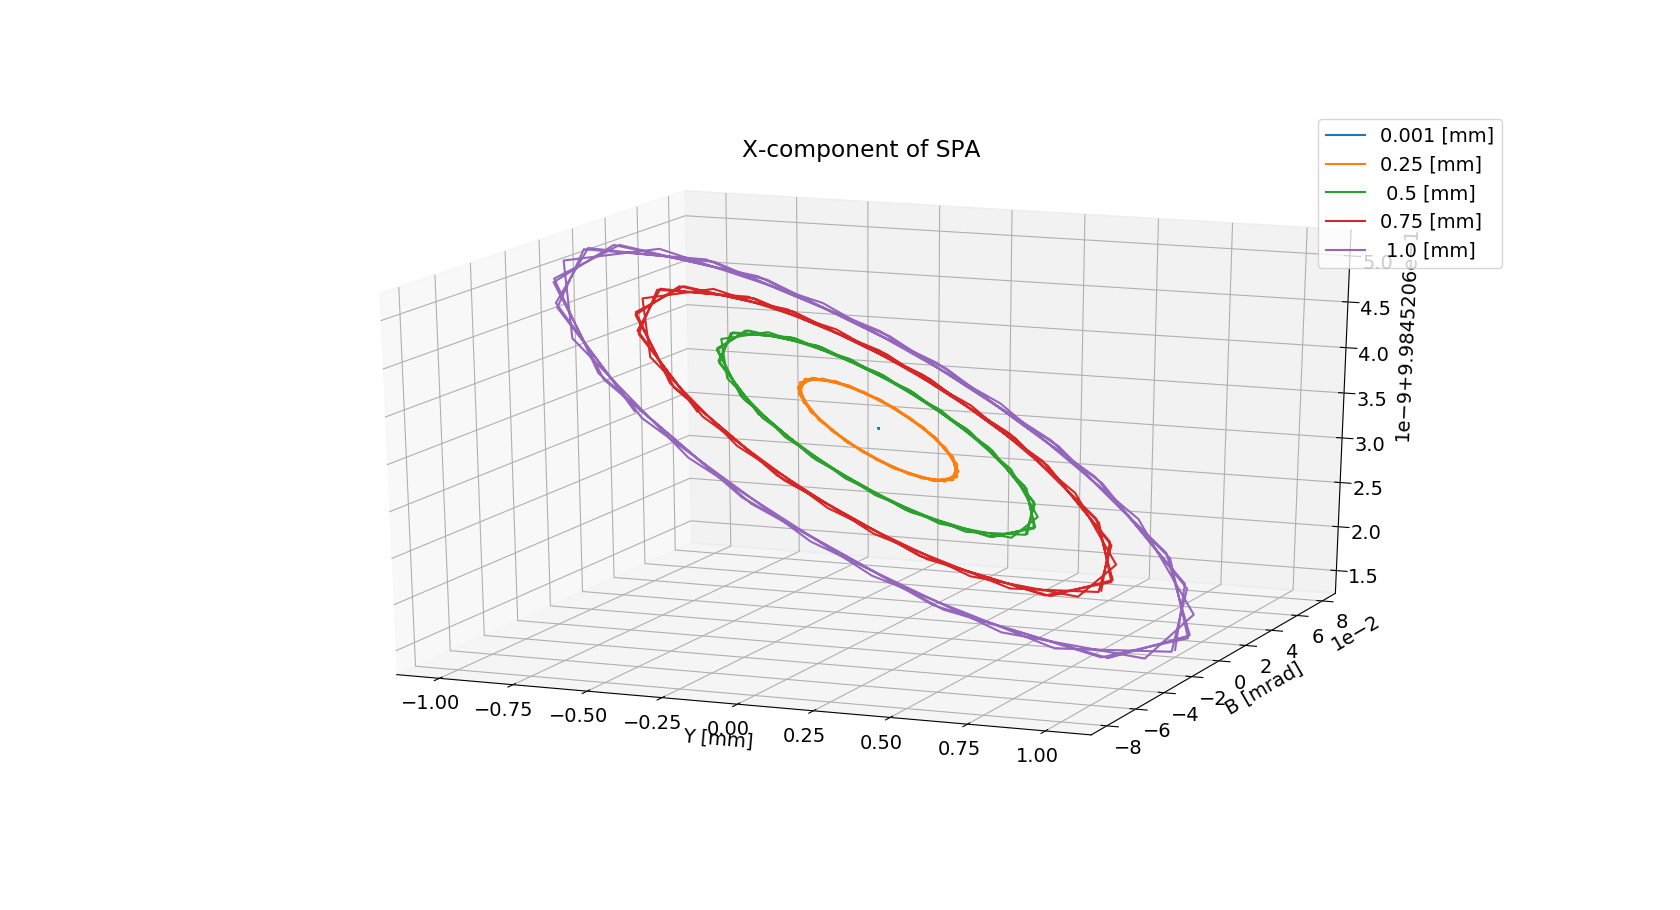
\includegraphics[width=\linewidth]{images/tss_on_betatron/nx}}
	\subbottom[Вертикальная компонента]{%
	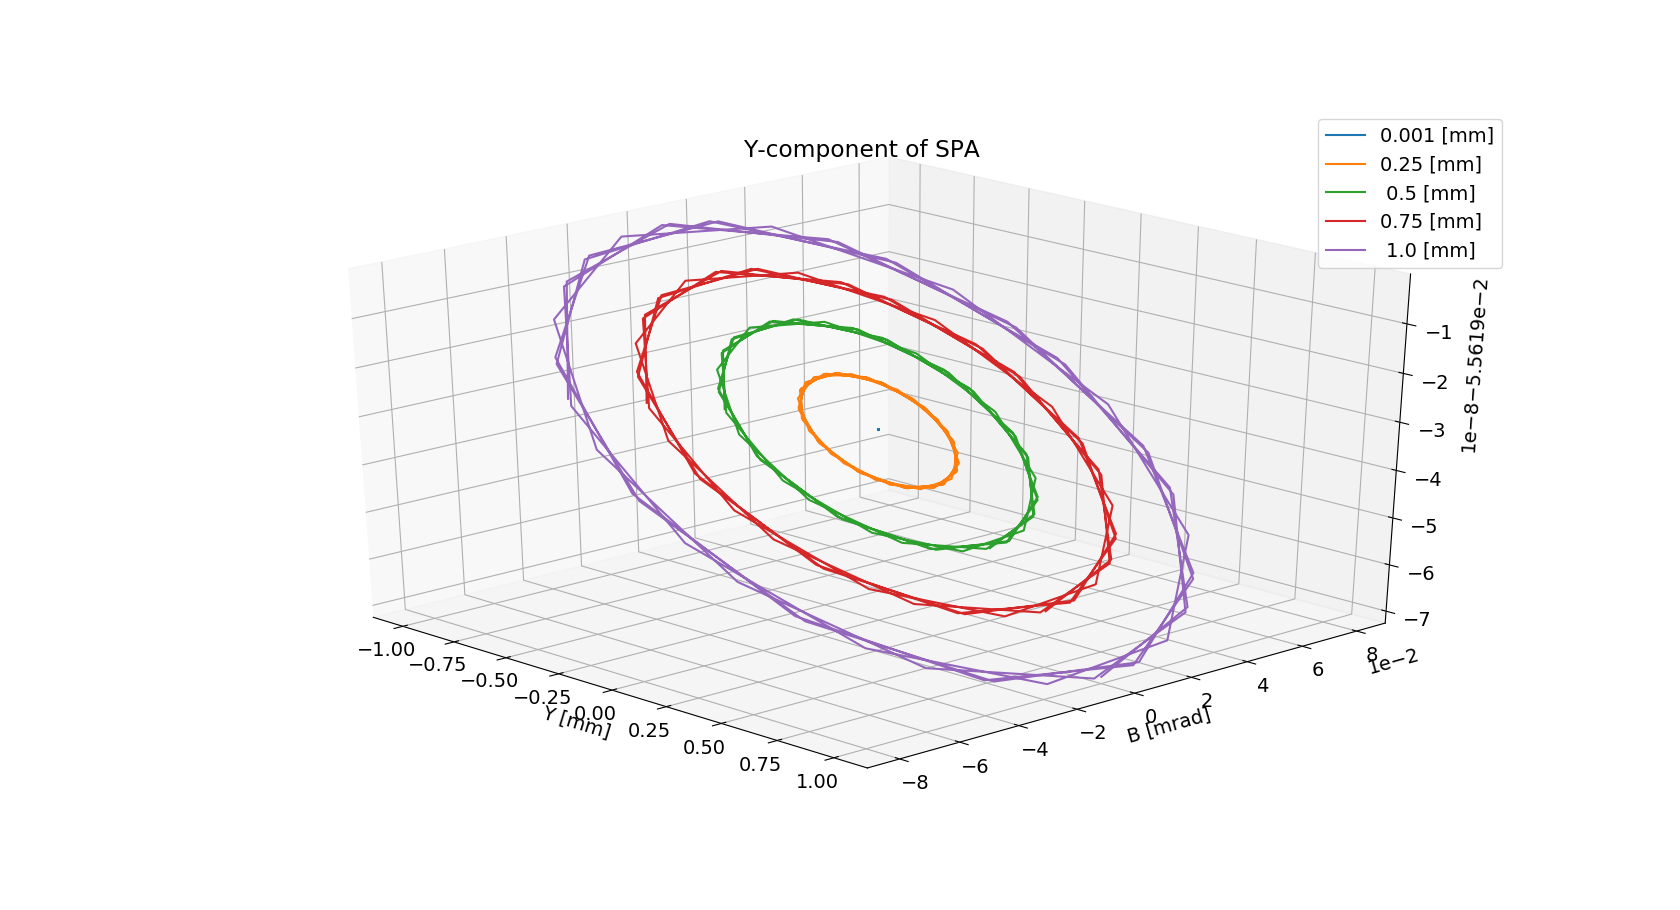
\includegraphics[width=\linewidth]{images/tss_on_betatron/ny}}
\end{figure}
\begin{figure}[h]
	\centering
	\contsubbottom[Продольная компонента]{%
		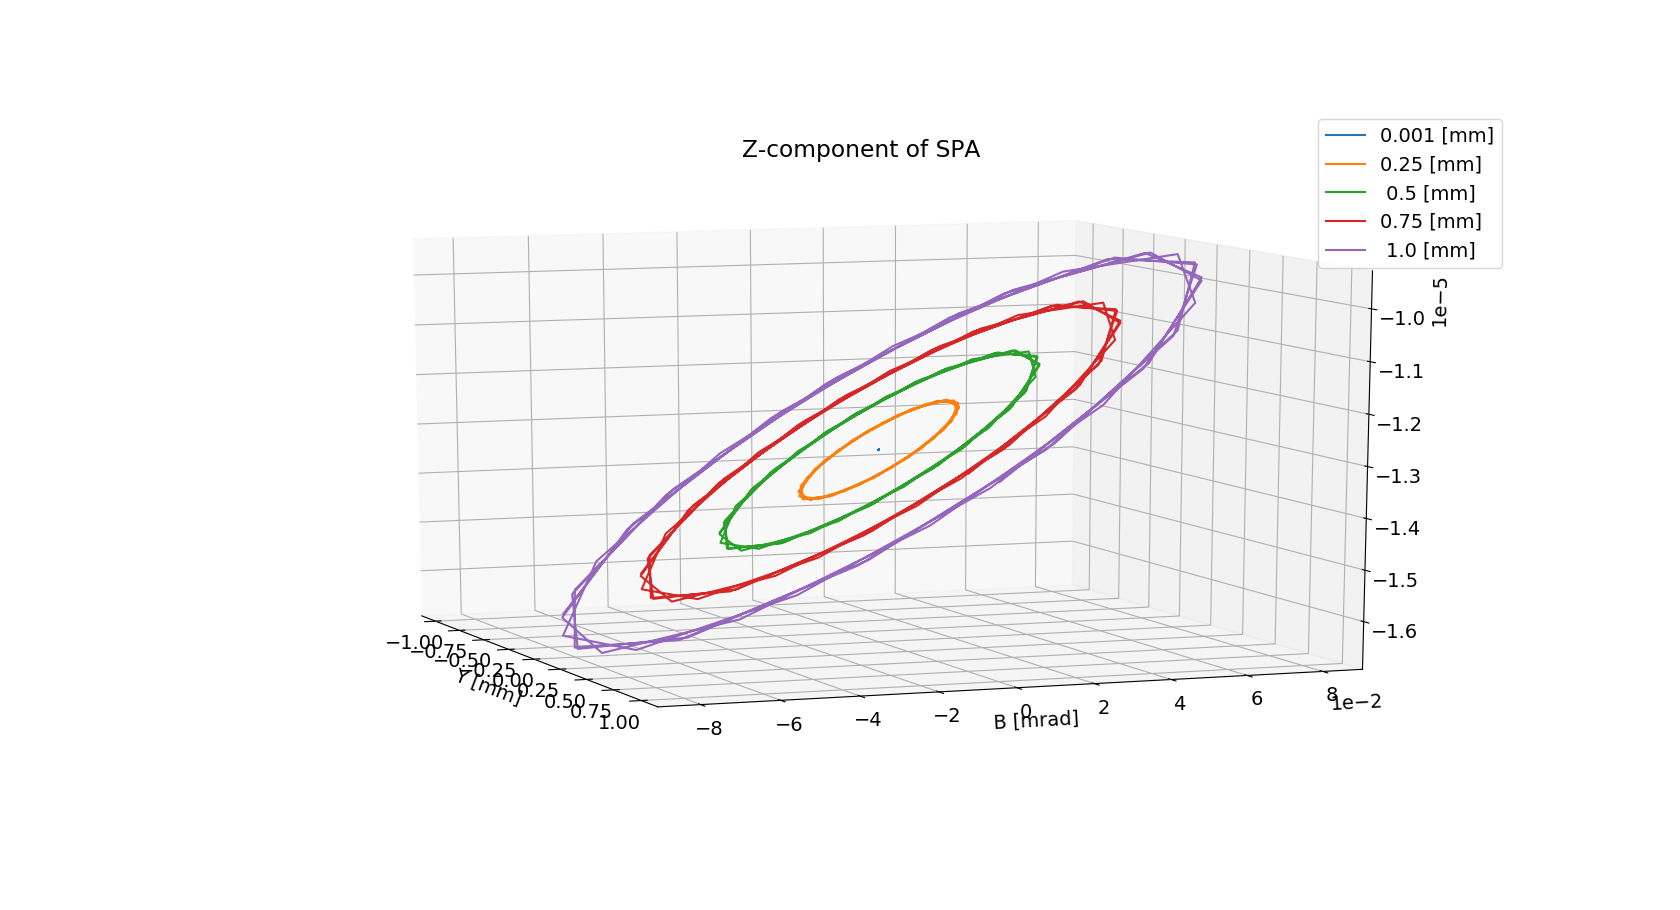
\includegraphics[width=\linewidth]{images/tss_on_betatron/nz}}
	\legend{Цветом обозначены частицы с различным начальным вертикальным смещением от референсной орбиты.}
	\caption{Компоненты оси прецессии спина, вычисленные на фазовых траекториях частиц, после применения секступольных полей для подавления эффекта декогеренции.\label{fig:n-bar_optimized}}
\end{figure}

\begin{figure}[h]
	\centering\hfill
	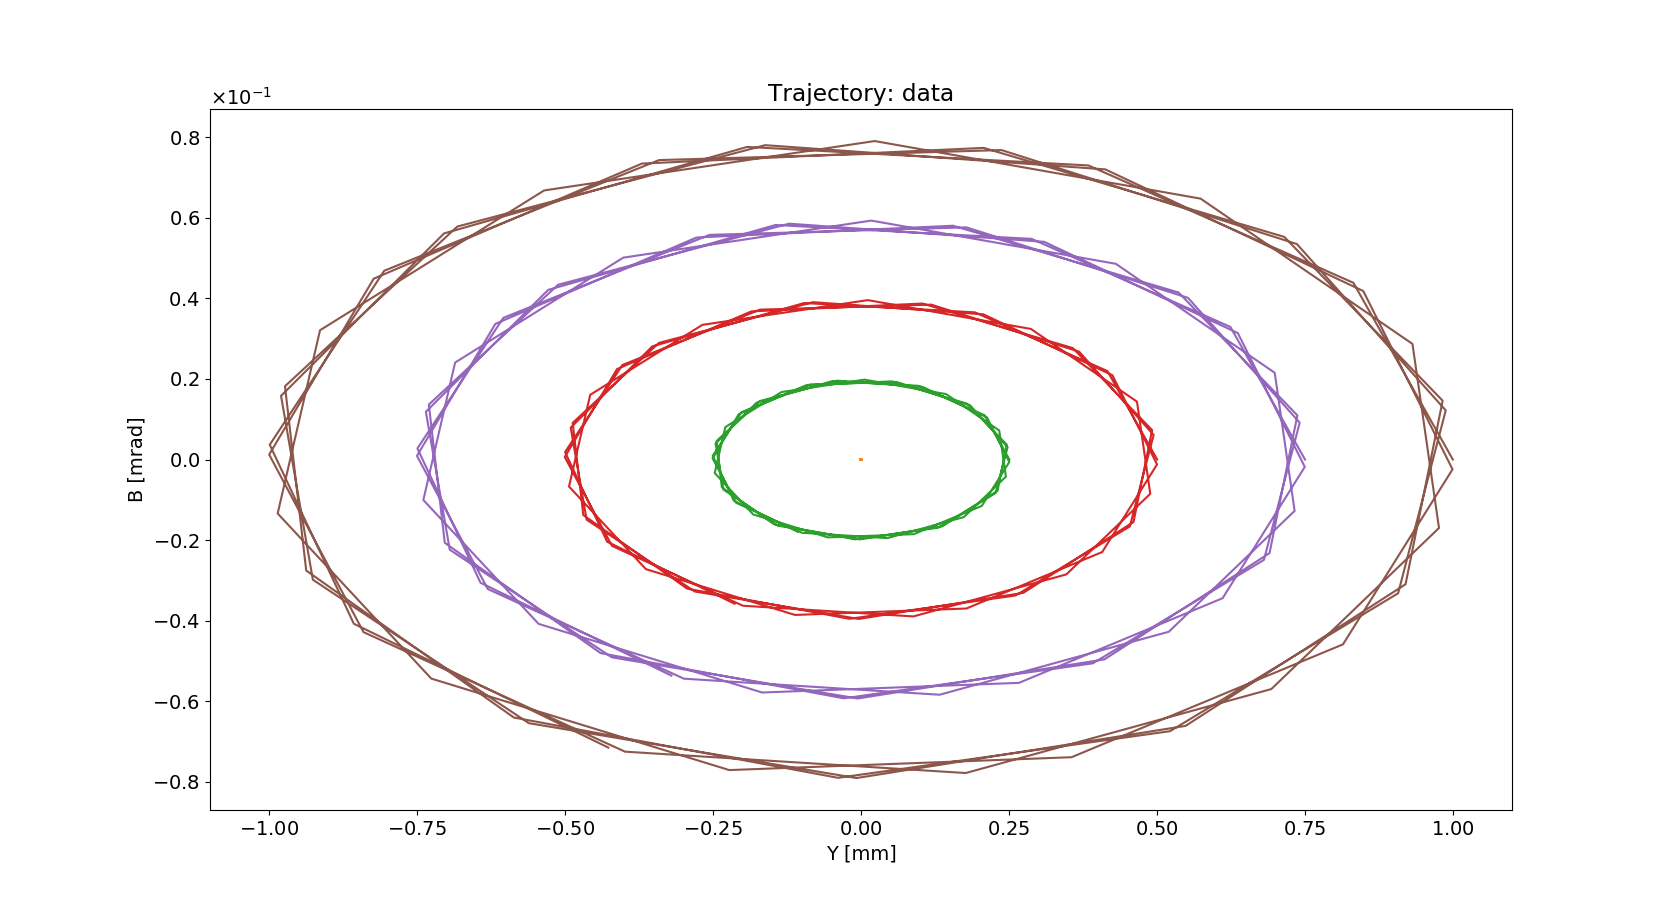
\includegraphics[width=\textwidth]{images/tss_on_betatron/phase_space}
	\caption{Фазовые траектории частиц в ускорителе.\label{fig:phase_space}}
\end{figure}

\begin{figure}[h]
	\centering
	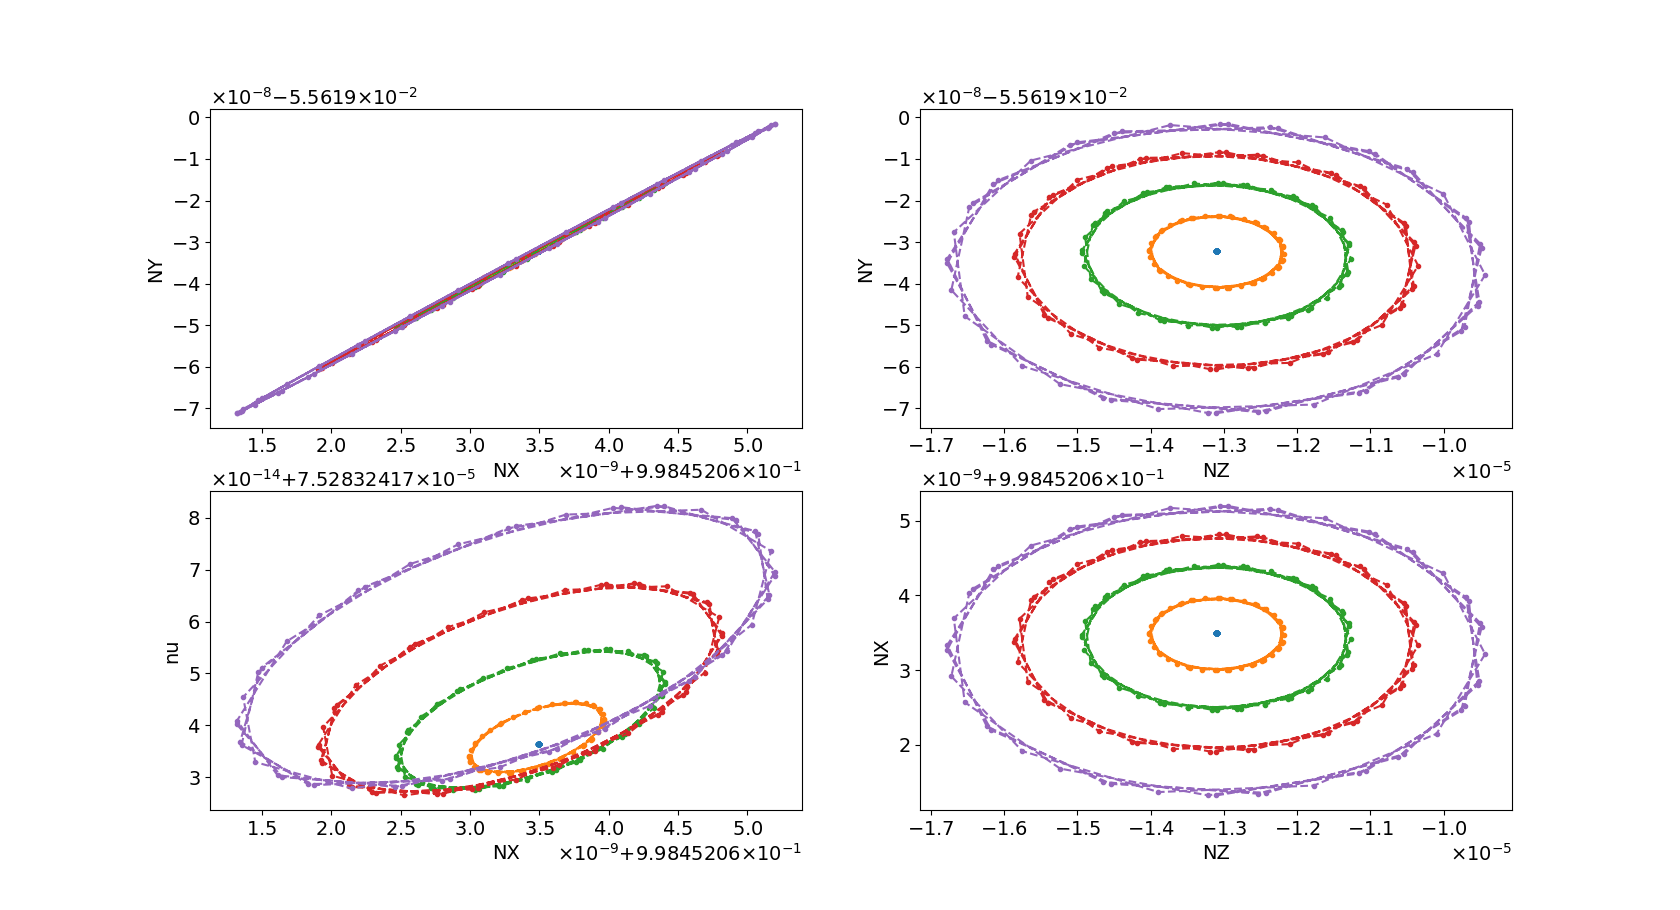
\includegraphics[width=\textwidth]{images/tss_on_betatron/all_vs_all}
	\caption{Компоненты спин-тюна и оси стабильного спина построенные друг против друга.\label{fig:all_vs_all}}
\end{figure}

\subsubsection{Симуляция}
Для подтверждения несущественности эффекта, была проведена следующая симуляция: был выбран ансамбль частиц, смещённых относительно рефернсной орбиты в вертикальном направлении в начальный момент времени. (Начальные значения всех остальных фазовых переменных равны нулю.)

Используя код COSY INFINITY мы протрекали этот ансамбль через структуру с замороженным спином (использующую секступольные поля для подавления декогеренции в вертикальной плоскости) на протяжении 1.2 миллиона оборотов (частота оборота пучка 1 МГц). Каждые 800 оборотов, процедурой TSS~\cite{COSYINF:BeamPhysMan} вычислялись разложения ряда Тейлора третьего порядка для $\nu_s(x,x',y,y',t,\delta)$ и $\bar n(x,x',y,y',t,\delta)$; затем вычислялись значения этих функций в точке фазового пространства, в которой на данный момент находилась частица. Таким образом были получены данные $(\nu_s(t), \bar n(t))$ частиц.

Далее эти данные были использованы для вычисления значений вертикальной компоненты спина $s_y^{func}(t)$ по формуле~\ref{eq:sy_varying_amplitude}. Также в процессе трекинга вычислялись значения $s_y^{data}(t)$ внутренними процедурами COSY INFINITY.

Затем обе серии фитировались функцией $y(t) = a\cdot \sin(2\pi\cdot f\cdot t + \phi)$, в которой оценивались все три параметра $(\hat a,\hat f,\hat \phi)$. Для оптимизации использовался алгоритм Левенберга-Марквардта.

\begin{table}[h]%
	\centering
	\changecaptionwidth\captionwidth{12cm}
	\caption{Результаты фитирования данных\label{tbl:smp-comparison}}
	\begin{tabular}{l|lcl}
		\toprule
		Данные & $\chi^2$ & AIC\footnotemark & $\hat f$, Гц\\
		\midrule
		$s_y^{func}$& $5.4\cdot 10^{-12}$& -49917& $74.452466548 \pm 1\cdot 10^{-9}$\\
		$s_y^{data}$& $2.0\cdot 10^{-6}$& -30665 & $74.452467 \pm 6\cdot 10^{-6}$\\\bottomrule
	\end{tabular}
\end{table}
\footnotetext{Информационный критерий Акаике. Поскольку AIC меньше для данных $s_y^{func}$, можно говорить, что они больше соответствуют синусоидальной модели с постоянной амплитудой и частотой, чем данные, полученные в результате трекинга.}

Исходя из результатов, представленных в Таблице~\ref{tbl:smp-comparison}, можно говорить о том, что прецессия оси стабильного спина не является основной причиной несоответствия данных синусоидальной модели.